\documentclass[norsk,a4paper,12pt]{article}
%\renewcommand{\thesection}{\Roman{section}} 
\usepackage[utf8]{inputenc}
\usepackage{graphicx} %for å inkludere grafikk
\usepackage{verbatim} %for å inkludere filer med tegn LaTeX ikke liker
\usepackage{tabularx}
\usepackage{booktabs}
\usepackage{amsmath}
\usepackage{float}
\usepackage{color}
\usepackage{listings}
\usepackage{hyperref}
\usepackage{csquotes}

\lstset{language=c++}
\lstset{basicstyle=\small}
\lstset{backgroundcolor=\color{white}}
\lstset{frame=single}
\lstset{stringstyle=\ttfamily}
\lstset{keywordstyle=\color{red}\bfseries}
\lstset{commentstyle=\itshape\color{blue}}
\lstset{showspaces=false}
\lstset{showstringspaces=false}
\lstset{showtabs=false}
\lstset{breaklines}
\lstset{postbreak=\raisebox{0ex}[0ex][0ex]{\ensuremath{\color{red}\hookrightarrow\space}}}
\usepackage{titlesec}

\setcounter{secnumdepth}{4}

\titleformat{\paragraph}
{\normalfont\normalsize\bfseries}{\theparagraph}{1em}{}
\titlespacing*{\paragraph}
{0pt}{3.25ex plus 1ex minus .2ex}{1.5ex plus .2ex}

\begin{document}

\begin{titlepage}
	\centering
	{\scshape\huge FYS4130 - Statistical Mechanics \par}
	\vspace{1cm}
	{\scshape\Large University of Oslo\par}
	\vspace{1.5cm}
	
\includegraphics[width=0.25\textwidth]{uio.png}\par\vspace{1cm}
	{\Large\bfseries Obligatory assignment\par}
	\vspace{1.5cm}
	{\large\itshape Even Marius Nordhagen\par}
	\vfill
	{\large \today\par}
\end{titlepage}


\section{CLUSTER SIZE}
This problem aims an one dimensional lattice with $N$ sites at a given temperature. There is a atom at each site that can either have energy $+\epsilon$ or $-\epsilon$, and a chain of sites with energy $+\epsilon$ is called a cluster.

\subsection{Onebody probabilities}
Since each atom can be in two possible energy states, the one-particle partition function has two terms
\begin{equation}
Z_1=\sum_ie^{-\beta\epsilon_i}=e^{-\beta\epsilon}+e^{\beta\epsilon}
\end{equation}
and the probability of an atom having energy $+\epsilon$ and $-\epsilon$ is
\begin{equation}
P_+=\frac{e^{-\beta\epsilon}}{Z_1}=\frac{e^{-\beta\epsilon}}{e^{-\beta\epsilon}+e^{\beta\epsilon}}\quad\text{and}\quad P_-=\frac{e^{\beta\epsilon}}{Z_1}=\frac{e^{\beta\epsilon}}{e^{-\beta\epsilon}+e^{\beta\epsilon}}
\end{equation}
respectively.

\subsection{Cluster number density}
The probability of finding a site at a specific position in a cluster of length $L$ is a function of the length and the occupation probability. For our purpose we denote the function as $n(L, P_+)$. Finding a site at a specific position in a cluster is just as probably as finding it in another cluster position, so the probability that a given site belongs to a cluster of length $L$ is 
\begin{equation}
P_L=Ln(L, P_+).
\end{equation}
$n(L, P_+)$ gives the probability of finding $L$ sites at energy $\epsilon$ and two sites at energy $-\epsilon$, 
\begin{equation}
n(L, P_+) = P_-^2\cdot P_+^L = (1-P_+)^2P_+^L
\end{equation}
because the site to the left of the cluster has energy $-\epsilon$ and so for the site to the right. We obtain 
\begin{equation}
P_L=L(1-P_+)^2P_+^L=L\bigg(\frac{e^{\beta\epsilon}}{e^{-\beta\epsilon}+e^{\beta\epsilon}}\bigg)^2\bigg(\frac{e^{-\beta\epsilon}}{e^{-\beta\epsilon}+e^{\beta\epsilon}}\bigg)^L
\end{equation}

\subsection{Normalization of the cluster number density}
We will now ensure that the sum over all cluster probabilities $P_L$ is $P_+$, which is a criteria since the probability of finding a site in a cluster of any size should be $P_+$. 
\begin{equation}
\sum_{L=1}^{\infty}P_L=\sum_{L=1}^{\infty}L(1-P_+)^2P_+^L=(1-P_+)^2P_+\sum_{L=1}^{\infty}LP_+^{L-1}
\label{PL}
\end{equation}
where $P_+^L$ is splitted up. We will now do a trick 
\begin{equation}
\sum_{x=1}^{\infty}xp^{x-1}=\frac{d}{dp}\sum_{x=0}^{\infty}p^x=\frac{d}{dp}\Big(\frac{1}{1-p}\Big)=\frac{1}{(1-p)^2}
\end{equation}
where we have used a common series. Setting back in equation [\ref{PL}], we find
\begin{equation}
(1-P_+)^2P_+\frac{1}{(1-P_+)^2}=P_+
\end{equation}
A cluster of length $L=0$ is not defined as a cluster, and the corresponding probability is therefore zero. 

\subsection{Average length of a cluster}
The average length of a cluster is given by
\begin{equation}
\langle L\rangle =\sum_{L=0}^{\infty}L^2(1-P_+)^2P_+^L
\end{equation}
from the general average statement for discrete values. We can let the sum run from $L=0$ because this just adds a zero term to the sum. 
\begin{align}
\langle L\rangle&=(1-P_+)^2\sum_{L=0}^{\infty}L^2P_+^L\\
&=(1-P_+)^2\bigg(\frac{P_+(P_++1)}{(1-P_+)^3}\bigg)\\
&=\frac{P_+(P_++1)}{1-P_+}\\
\end{align}
where we again have replaced the sum with the known answer. We can now insert the onebody probabilities. Observe that the denominator is  $P_-$ and $P_+/P_-=e^{-2\beta\epsilon}$, and get
\begin{align}
\langle L\rangle=e^{-2\beta\epsilon}\bigg(\frac{e^{\beta\epsilon}+2e^{-\beta\epsilon}}{e^{\beta\epsilon}+e^{-\beta\epsilon}}\bigg).
\end{align}
The average length is plotted as a function of the temperature in figure [\ref{y_time}], and we see that the average length decreases rapidly when $T\rightarrow0$. The low-temperature limit is not very informative when we already know that the average length goes to zero when the temperature approaches zero, but it is interesting to see what the high-temperature asymptote is. 

\begin{figure}[h]
\centering
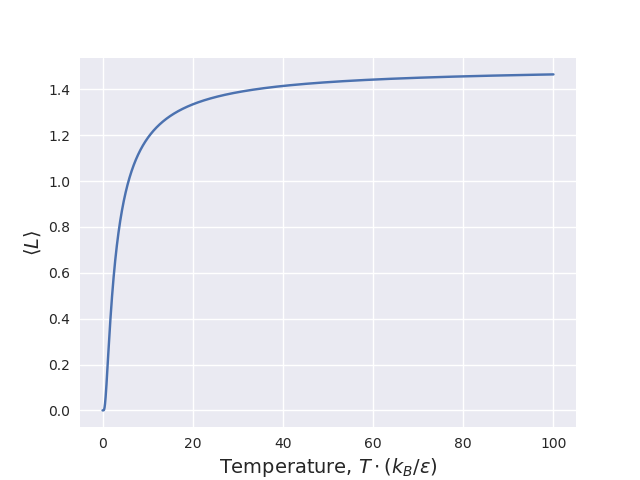
\includegraphics[width=150mm]{1_4.png}
\caption{Average length of cluster as a function of temperature. In this plot the temperature spans from 0 to 100 given in units of $\epsilon/k_B$ where $k_B$ is Boltzmanns constant. \label{y_time}}
\end{figure}

The high-temperature limit is
\begin{equation}
\lim_{T\rightarrow\infty}\langle L\rangle = 1\bigg(\frac{1+2}{1+1}\bigg)=\frac{3}{2}
\end{equation}
which matches the plot. The low-temperature limit is
\begin{equation}
\lim_{T\rightarrow\infty}\langle L\rangle = \lim_{T\rightarrow\infty} \frac{1+2e^{-2\epsilon/kT}}{1+e^{2\epsilon/kT}}=\frac{1+0}{1+\infty}=0.
\end{equation}
as expected. We can connect these numbers to the onebody probabilities, which can be rewritten as
\begin{equation}
P_+=\frac{1}{1+e^{2\beta\epsilon}}\quad\text{and}\quad P_-=\frac{1}{1+e^{-2\beta\epsilon}}.
\end{equation}
When $T\rightarrow 0$ all the sites will have energy $-\epsilon$, and we will not have any clusters (therefore the average cluster length goes to zero). On the other hand, when $T\rightarrow\infty$, an equal number of sites have energy $\epsilon$ as having $-\epsilon$, and the most likely configurations give an average cluster length between 1 and 2.

\newpage
\section{ELECTRON GAS IN A MAGNETIC FIELD}
Here we study an electron gas in a magnetic field, where each particular electron has energy $\varepsilon_T=\varepsilon\mp\mu_BH$ depending on whether its magnetic moment is parallel or antiparallel to the field. $\varepsilon_T$ is the total energy of an electron, $\varepsilon$ is its kinetic energy and $\pm\mu_BH$ is the magnetic energy. 

\subsection{Average number of particles}
For continuous energies, the average number of fermions with infinitesimal energy $d\varepsilon$ is
\begin{equation}
dN(\varepsilon)=g(\varepsilon)\bar{n}(\varepsilon_T)d\varepsilon
\end{equation}
and the average total number of particles is 
\begin{equation}
\langle N\rangle=\int_0^{\infty}d\varepsilon g(\varepsilon)\bar{n}(\varepsilon_T).
\end{equation}
Notice that the density function $g(\varepsilon)$ takes the kinetic energy, while the distribution function $\bar{n}(\varepsilon_T)$ takes the total energy. The electrons are Fermi-Dirac distributed and in our case the density of states is
$g(\varepsilon)=AV\varepsilon^{1/2}$ with $A=(2/\sqrt{\pi})(2\pi m/\hbar^2)^{3/2}$, such that 
\begin{equation}
\langle N\rangle=AV\int_0^{\infty}d\varepsilon\frac{\varepsilon^{1/2}}{e^{\beta(\varepsilon_T-\mu)+1}}.
\end{equation}
When inserting for the total energy, we need to seperate the average depending on whether the magnetic energy is positive or negative. We get
\begin{equation}
\langle N_{\pm}\rangle=AV\int_0^{\infty}d\varepsilon\frac{\varepsilon^{1/2}}{e^{\beta(\varepsilon\mp\mu_BH-\mu)+1}}
\end{equation}
where we can define $x=\mu\pm\mu_BH$. The integral is quite tricky, but we can express it in terms of the Sommerfeld expansion:
\begin{equation}
\int_0^{\infty}d\varepsilon\frac{\varepsilon^{1/2}}{e^{\beta(\varepsilon-x)+1}}\cong\frac{2}{3}x^{3/2}+\frac{\pi^2}{12}(kT)^2x^{-1/2}+\hdots
\end{equation}
shown in the appendix. We are left with
\begin{equation}
\langle N_{\pm}\rangle=\frac{2V}{\sqrt{\pi}}\bigg(\frac{2\pi m}{\hbar^2}\bigg)^{3/2}\bigg(\frac{2}{3}(\mu\pm\mu_BH)^{3/2}+\frac{\pi^2}{12}(kT)^2(\mu\pm\mu_BH)^{-1/2}\bigg)
\end{equation}
MIGHT PLOT AVERAGES

\subsection{Average magnetization}
The average magnetization is given by
\begin{align}
\langle M\rangle&=\mu_B(\langle N_-\rangle-\langle N_+\rangle)\\
&
\begin{aligned}
=AV\mu_B\bigg(\frac{2}{3}&\Big((\mu-\mu_BH)^{3/2}-(\mu+\mu_BH)^{3/2}\Big)+\\
\frac{\pi^2}{12}(kT)^2&\Big((\mu-\mu_BH)^{-1/2}-(\mu+\mu_BH)^{-1/2}\Big)\bigg)
\end{aligned}
\end{align}
inserted the expression from previous exercise. For small temperatures the second line vanishes, and 

\newpage
\section{QUANTUM COULOMB GAS}
We will look at a relativistic quantum gas of positive and negative charged particles with coulomb interaction. In addition we have an external box potential with walls of length $L$. Although we cannot solve this analytically, we will get some results. The given Hamiltonian is as follows
\begin{equation}
{\cal H}=\sum_{i=1}^{2N}c|\boldsymbol{p}_i|+\sum_{i<j}^{2N}\frac{e_ie_j}{|\boldsymbol{r}_i - \boldsymbol{r}_j|}
\end{equation}

\subsection{Schrödinger equation}
The general Schrödinger equation for a many-body system is 
\begin{equation}
H\Psi_n=E_n\Psi_n
\end{equation}
where $\Psi_n$ is the total wave function of state $n$ and $E_n$ is the corresponding total energy. The wave functions are position dependent and the energies are dependent on the box size,
\begin{equation}
{\cal H}\Psi_n(\{\boldsymbol{r}_i\})=\epsilon_n(L)\Psi_n(\{\boldsymbol{r}_i\}).
\end{equation}
The exact wave functions are unknown, but there are some constraints that apply in general. Since the particles are indistinguishable, all observable should be the same although we swap two coordinates. This results in
\begin{equation}
P(a,b)=P(b,a)\quad\Rightarrow\quad |\Psi(a,b)|^2=|\Psi(b,a)|^2
\end{equation}
and
\begin{equation}
\Psi(a,b)=e^{i\phi}\Psi(b,a).
\end{equation}
Swapping twice must give back the initial wave function, so there are two possible choices of $\phi$: 0 and $2\pi$. The first one gives a symmetric total wavefunction under exchange of two particles, which is antisymmetric for the second choice. We denote the former as bosons and the latter as fermions, where the Pauli principle is a consequence of antisymmetry.

\subsection{Scaling}
We will now scale the coordinates with respect to $L$ such that the box gets size $1^d$ where $d$ is the number of dimensions, matematically written as
\begin{equation}
\boldsymbol{r}_i'=\boldsymbol{r}_i/L.
\end{equation}
Using that the operator of linear momentum is given by 
\begin{equation}
\boldsymbol{p}_i=-i\hbar\nabla_i=-i\hbar\Big(\frac{\partial}{\partial x_1},\frac{\partial}{\partial x_2},\hdots,\frac{\partial}{\partial x_d}\Big),
\end{equation}
the corresponding scaled momentum operator is 
\begin{equation}
\boldsymbol{p}_i'=-i\hbar\Big(\frac{\partial}{\partial x_1'},\frac{\partial}{\partial x_2'},\hdots,\frac{\partial}{\partial x_d'}\Big)= \frac{\boldsymbol{p}_i}{L}
\end{equation}
which is the scaling of the first term of the Hamiltonian. The second term is scaled similarly, and by denoting the scaled Hamiltonian as ${\cal H}'$, we get ${\cal H}={\cal H}'/L$. We are now set to scale the Schrödinger equation, which becomes
\begin{equation}
\frac{{\cal H}'}{L}\Psi_n(\{\boldsymbol{r}_i\})=\frac{\epsilon_n(1)}{L}\Psi_n(\{\boldsymbol{r}_i\})
\end{equation}
where the scaled energy is a function of 1 since the length scale now is 1, such that $\epsilon_n(L)=\epsilon_n(1)/L$.

\subsection{Collapse V + T}
We have a fixed number of particles and the energy cna fluctuate, so we are in the canonical ensemble. The one particle partition function is given by
\begin{equation}
Z_1=\sum_{n=0}^{\infty}e^{-\beta\epsilon_n(L)}
\end{equation}
which in three dimensions is given by
\begin{align}
Z_1(V,T)&=\sum_{n_x,n_y,n_z=0}^{\infty}\exp{\big(-\beta\epsilon_{n_x}(L)\epsilon_{n_y}(L)\epsilon_{n_z}(L)}\big)\\
&=\sum_{n_x,n_y,n_z=0}^{\infty}\exp\Big({-\frac{\epsilon_{n_x}(1)\epsilon_{n_y}(1)\epsilon_{n_z}(1)}{k^3T^3L^3}}\Big).
\end{align}
Since $L^3=V$, the one particle partition function is a function of $VT^3$. The total partition function is given by 
\begin{equation}
Z(N,V,T)=\frac{Z_1(V,T)^N}{N!}=\frac{1}{N!}\sum_{n_{\boldsymbol{k}}=0}^{\infty}e^{-N\frac{\epsilon_{n_{\boldsymbol{k}}}(1)}{k^3VT^3}}={\cal Z}(N,VT^3)
\end{equation}
since the particles are indistinguishable.

\subsection{Energy and pressure relation}
The internal energy in this system is a sum over all energy levels times the probability of that level. Further we observe that we can differentiate the exponential with respect to $\beta$ to obtain the same expression,
\begin{equation}
E=\frac{1}{Z}\sum_n\epsilon_ne^{-\beta\epsilon_n}=-\frac{1}{Z}\sum_n\frac{\partial}{\partial\beta}e^{-\beta\epsilon_n}=-\frac{1}{Z}\frac{\partial Z}{\partial\beta}.
\end{equation}
The pressure is given by the differential
\begin{equation}
P(N,V)=-\Big(\frac{\partial F}{\partial V}\Big)_N
\end{equation}
where $F$ is Helmholtz free energy,
\begin{equation}
F=-kT\ln Z.
\end{equation}
We therefore end up with the expressions 
\begin{align}
E&=-\frac{1}{Z}\frac{\partial Z}{\partial\beta}\\
P&=kT\frac{1}{Z}\frac{\partial Z}{\partial V}
\end{align}
such that they are related through the partition function. We use the same partition function as we found in the previous exercise, and obtain
\begin{align}
\frac{\partial Z}{\partial \beta}&=-3\frac{\beta^2\epsilon_{n_{\boldsymbol{k}}}(1)}{V}Z\\
\frac{\partial Z}{\partial V}&=\frac{\beta^3\epsilon_{n_{\boldsymbol{k}}}(1)}{V^2}Z.
\end{align}
The energy then reads
\begin{equation}
E=3\frac{\beta^2\epsilon_{n_{\boldsymbol{k}}}(1)}{V}=3kT\frac{\beta^3\epsilon_{n_{\boldsymbol{k}}}(1)}{V^2}V=3PV.
\end{equation}

Notice that the calculations are done for the one particle partition function, but it is easy to imagine that the full partition function will give the same result. 

\subsection{Non-relativistic gas}
We now switch from a relativistic gas to a non-relativistic one and redo the exercises in four dimensions. The Hamiltonian is then given by
\begin{equation}
{\cal H}=\sum_{i=1}^{2N}\frac{\boldsymbol{p}_i^2}{2m}+\sum_{i<j}^{2N}\frac{e_ie_j}{|\boldsymbol{r}_i - \boldsymbol{r}_j|}.
\end{equation}
We then do a change of scale similarly as in exercise 3.2, and get the Schrödinger equation 
\begin{equation}
\frac{{\cal H}'}{L^2}\Psi_n(\{\boldsymbol{r}_i\})=\frac{\epsilon_n(1)}{L^2}\Psi_n(\{\boldsymbol{r}_i\})
\end{equation}
where  ${\cal H}'$ is the scaled Hamiltonian. Further the partition function is 
\begin{align}
Z_1&=\sum_{n_x,n_y,n_z,n_u=0}^{\infty}\exp\Big({-\beta^4\epsilon_{n_x}(L)\epsilon_{n_y}(L)\epsilon_{n_z}(L)\epsilon_{n_u}(L)}\Big)\\
&=\sum_{n_x,n_y,n_z,n_u=0}^{\infty}\exp\Big({-\frac{\beta^4\epsilon_{n_x}(1)\epsilon_{n_y}(1)\epsilon_{n_z}(1)\epsilon_{n_u}(1)}{L^8}}\Big)
\end{align}
and since we are in 4D, the 4-volume is $V_4=L^4$. We can reuse the expressions for energy and pressure from above, and find a relation between the energy and pressure as we did in exercise 3.4. Again we calculate the differentials
\begin{align}
\frac{\partial Z}{\partial \beta}&=-4\frac{\beta^3\epsilon_{n_{\boldsymbol{k}}}(1)}{V_4^2}Z\\
\frac{\partial Z}{\partial V_4}&=2\frac{\beta^4\epsilon_{n_{\boldsymbol{k}}}(1)}{V_4^3}Z.
\end{align}
and find the relation
\begin{equation}
E=4\frac{\beta^3\epsilon_{n_{\boldsymbol{k}}}(1)}{V_4^2}=4kT\frac{\beta^4\epsilon_{n_{\boldsymbol{k}}}(1)}{V_4^3}=2PV
\end{equation}.

Again this is results is found from the one particle partition function, but it is general for a non-relativistic interacting quantum gas in 4D.

\newpage
\section{NON-INTERACTING FERMIONS}
In this problem we study a non-interacting fermi gas with chemical potential $\mu$. The particle states are given by the vector $\vec{k}$, which is $d$-dimensional where $d$ is number of spatial dimensions, and the corresponding energy is $\epsilon(\vec{k})$.

\subsection{Joint probability}
The joint probability of finding a particle in a state given by the occupation numbers $\{n_{\vec{k}}\}$ is given by a product of the general probability statement in a grand canonical ensemble (hence joint),
\begin{equation}
P(\{n_{k}\})=\frac{\prod_ke^{-\beta n_k(\epsilon_k-\mu)}}{\Xi},
\end{equation}
where $\Xi$ is the grand canonical partition function, given by
\begin{align}
\Xi&=\sum_{\{n_k\}}\prod_k\exp\big(-\beta(\epsilon_k-\mu)n_k\big)\\
&=\prod_k\sum_{n_k=0}^1\exp\big(-\beta(\epsilon_k-\mu)n_k\big)\\
&=\prod_k\Big(1+\exp\big(-\beta(\epsilon_k-\mu)\big)\Big)
\end{align}
since we only can have 0 or 1 fermion in each energy state according to the Pauli principle. 
\begin{equation}
P(\{n_{k}\})=\frac{\prod_ke^{-\beta n_k(\epsilon_k-\mu)}}{\prod_k\big(1+e^{-\beta(\epsilon_k-\mu)}\big)}=\prod_k\frac{e^{\beta n_k(\mu-\epsilon_k)}}{1+e^{\beta(\mu-\epsilon_k)}}
\end{equation}

\subsection{Average occupation number}
The average occupation number of a state is given by Fermi-Dirac distribution
\begin{equation}
\langle n_k\rangle = \frac{1}{e^{\beta(\epsilon_k-\mu)}+1}.
\end{equation}
We can easily write the probability as a function of $\langle n_k\rangle$ ,
\begin{align}
P(\{n_{k}\})&=\prod_k\frac{e^{\beta(\epsilon_k-\mu)(1-n_k)}}{e^{\beta(\epsilon_k-\mu)}}\\
&=\prod_k\langle n_k\rangle e^{\beta(\epsilon_k-\mu)(1-n_k)}\\
&=\prod_k\langle n_k\rangle \frac{e^{\beta(\epsilon_k-\mu)}}{e^{\beta(\epsilon_k-\mu)n_k}}
\end{align}

\subsection{Maximum entropy of random variable}
A random variable has $l$ discrete outcomes with their own respective probabilities. Since the probabilities are independent, we can find the information entropy
\begin{equation}
S=H(p_1,\hdots,p_n)=-\sum_{n=1}^lp_n\log p_n
\label{entropy}
\end{equation}
where $p_i$ is the probability of outcome $i$. We cannot find the exact entropy without knowing the probabilities, but we can find which probabilities that give maximum entropy. For this we use Lagrange multipliers with the normalization condition as the constraint,
\begin{equation}
\sum_{n=1}^Lp_n=1\quad\Rightarrow\quad G(p_1,\hdots,p_l)=\sum_{n=1}^Lp_n-1=0.
\end{equation}
The Lagrangian is thus given by
\begin{align}
{\cal L}(p_1,\hdots,p_l,\lambda)&=H(p_1,\hdots,p_l)+\lambda\cdot G(p_1, \hdots,p_l)\\
&=-\sum_{n=1}^lp_n\log p_n + \lambda\Big(\sum_{n=1}^lp_n-1\Big)
\end{align}
which we maximize to find the maximum entropy. The gradient with respect to all variables is
\begin{equation}
\nabla_{p_1,\hdots,p_l,\lambda}{\cal L}(p_1,\hdots,p_l,\lambda)=\bigg(\frac{\partial {\cal L}}{\partial p_1},\hdots,\frac{\partial {\cal L}}{\partial p_l},\frac{\partial {\cal L}}{\partial \lambda}\bigg)
\end{equation}
\begin{equation}
\frac{\partial {\cal L}}{\partial p_j}=-\log p_j-1+\lambda,\quad\quad\quad \frac{\partial {\cal L}}{\partial \lambda}=\sum_{n=1}^lp_n-1
\end{equation}
which is maximized when $\nabla{\cal L}=\vec{0}$. This occur when 
\begin{equation}
p_j=e^{\lambda-1}=\frac{1}{l}=P
\end{equation}
such that all probabilities are equal and $P=1/l$ due to the normalization. The information entropy is therefore maximized as
\begin{equation}
S=-lP\log P=\log l
\end{equation}
This also matches to the principle of maximum entropy, which states that
\begin{displayquote}
"If nothing is known about a distribution except that it belongs to a certain class, then the distribution with the largest entropy should be chosen as the least-informative default".
\end{displayquote}
The least-informative default is clearly when all probabilities are equal.

\subsection{Entropy of fermi gas}
We will now find the entropy of the gas discussed in exercises 4.1 and 4.2. Recall the average occupation number
\begin{equation}
\langle n_k\rangle = \frac{1}{e^{\beta(\epsilon_k-\mu)}+1}=\frac{n_k}{g_k}
\label{entropy}
\end{equation}
where $n_k$ is the total number of particles and $g_k$ is the... WRITE HERE
A fermi gas has in general a number of avaliable states given by
\begin{equation}
W=\prod_k\frac{g_k!}{n_k!(g_k-n_k)!}.
\end{equation}
We can then find the (Boltzmann) entropy by
\begin{align}
S&=k\log W\\
&=k\sum_k\log\bigg(\frac{g_k!}{n_k!(g_k-n_k)!}\bigg)\\
&=k\sum_kg_k\bigg(\log g_k-\frac{n_k}{g_k}\log n_k-\Big(1-\frac{n_k}{g_k}\Big)\Big(\log g_k + log\big(1-\frac{n_k}{g_k}\big)\Big)\bigg)\\
&=k\sum_kg_k\Big(-\langle n_k\rangle\log\langle n_k\rangle+\big(1-\langle n_k\rangle\big)\log\big(1-\langle n_k\rangle\big)\Big)
\end{align}
where Sterling's approximation is applied. The avergae occupation number from equation [\ref{entropy}] can now be inserted, and we get
\begin{equation*}
S=k\sum_kg_k\bigg(\log(e^{-\beta(\epsilon_k-\mu)}+1)+\frac{\log(e^{\beta(\epsilon_k-\mu)}+1)-\log(e^{-\beta(\epsilon_k-\mu)}+1)}{e^{\beta(\epsilon_k -\mu)}+1}\bigg)
\end{equation*}
For the low-temperature limit some terms vanish and we are left with
\begin{equation}
\lim_{T\rightarrow 0}S=\frac{\log(e^{\beta(\epsilon_k-\mu)}+1)}{e^{\beta(\epsilon_k -\mu)}}
\end{equation}
which is a "$\infty/\infty$-expression". We solve it by L'Hôpital's rule:
\begin{align}
\lim_{T\rightarrow 0}S&=k\sum_kg_k\frac{\frac{d}{dT}\log(e^{\beta(\epsilon_k-\mu)}+1)}{\frac{d}{dT}e^{\beta(\epsilon_k -\mu)}}\\
&=k\sum_kg_k\frac{(e^{\beta(\epsilon_k-\mu)}+1)^{-1}\cdot\big(-\frac{1}{kT^2}(\epsilon_k-\mu)\big)e^{\beta(\epsilon_k-\mu)}}{\big(-\frac{1}{kT^2}(\epsilon_k-\mu)\big)e^{\beta(\epsilon_k-\mu)}}\\
&=k\sum_k\frac{g_k}{e^{\beta(\epsilon_k-\mu)}+1}
\end{align}
which again is the Fermi-Dirac distribution. At zero temperature this is a step function where there are no occupied states above the Fermi energy. 

\end{document}
